	%Version 3 October 2023
% See section 11 of the User Manual for version history
%
%%%%%%%%%%%%%%%%%%%%%%%%%%%%%%%%%%%%%%%%%%%%%%%%%%%%%%%%%%%%%%%%%%%%%%
%%                                                                 %%
%% Please do not use \input{...} to include other tex files.       %%
%% Submit your LaTeX manuscript as one .tex document.              %%
%%                                                                 %%
%% All additional figures and files should be attached             %%
%% separately and not embedded in the \TeX\ document itself.       %%
%%                                                                 %%
%%%%%%%%%%%%%%%%%%%%%%%%%%%%%%%%%%%%%%%%%%%%%%%%%%%%%%%%%%%%%%%%%%%%%
%%\documentclass[referee,sn-basic]{sn-jnl}% referee option is meant for double line spacing

%%=======================================================%%
%% to print line numbers in the margin use lineno option %%
%%=======================================================%%

%%\documentclass[lineno,sn-basic]{sn-jnl}% Basic Springer Nature Reference Style/Chemistry Reference Style

%%======================================================%%
%% to compile with pdflatex/xelatex use pdflatex option %%
%%======================================================%%

%%\documentclass[pdflatex,sn-basic]{sn-jnl}% Basic Springer Nature Reference Style/Chemistry Reference Style


%%Note: the following reference styles support Namedate and Numbered referencing. By default the style follows the most common style. To switch between the options you can add or remove �Numbered� in the optional parenthesis. 
%%The option is available for: sn-basic.bst, sn-vancouver.bst, sn-chicago.bst%  

%%\documentclass[sn-nature]{sn-jnl}% Style for submissions to Nature Portfolio journals
%%\documentclass[sn-basic]{sn-jnl}% Basic Springer Nature Reference Style/Chemistry Reference Style
\documentclass[sn-mathphys-num]{sn-jnl}% Math and Physical Sciences Numbered Reference Style 
%%\documentclass[sn-mathphys-ay]{sn-jnl}% Math and Physical Sciences Author Year Reference Style
%%\documentclass[sn-aps]{sn-jnl}% American Physical Society (APS) Reference Style
%%\documentclass[sn-vancouver,Numbered]{sn-jnl}% Vancouver Reference Style
%%\documentclass[sn-apa]{sn-jnl}% APA Reference Style 
%%\documentclass[sn-chicago]{sn-jnl}% Chicago-based Humanities Reference Style

%%%% Standard Packages
%%<additional latex packages if required can be included here>

\usepackage{graphicx}%
\usepackage{multirow}%
\usepackage{amsmath,amssymb,amsfonts}%
\usepackage{amsthm}%
\usepackage{mathrsfs}%
\usepackage[title]{appendix}%
\usepackage{xcolor}%
\usepackage{textcomp}%
\usepackage{manyfoot}%
\usepackage{booktabs}%
\usepackage{algorithm}%
\usepackage{algorithmicx}%
\usepackage{algpseudocode}%
\usepackage{listings}%
\usepackage{subcaption}


%%%%

%%%%%=============================================================================%%%%
%%%%  Remarks: This template is provided to aid authors with the preparation
%%%%  of original research articles intended for submission to journals published 
%%%%  by Springer Nature. The guidance has been prepared in partnership with 
%%%%  production teams to conform to Springer Nature technical requirements. 
%%%%  Editorial and presentation requirements differ among journal portfolios and 
%%%%  research disciplines. You may find sections in this template are irrelevant 
%%%%  to your work and are empowered to omit any such section if allowed by the 
%%%%  journal you intend to submit to. The submission guidelines and policies 
%%%%  of the journal take precedence. A detailed User Manual is available in the 
%%%%  template package for technical guidance.
%%%%%=============================================================================%%%%

%% as per the requirement new theorem styles can be included as shown below
\theoremstyle{thmstyleone}%
\newtheorem{theorem}{Theorem}%  meant for continuous numbers
%%\newtheorem{theorem}{Theorem}[section]% meant for sectionwise numbers
%% optional argument [theorem] produces theorem numbering sequence instead of independent numbers for Proposition
\newtheorem{proposition}[theorem]{Proposition}% 
%%\newtheorem{proposition}{Proposition}% to get separate numbers for theorem and proposition etc.

\theoremstyle{thmstyletwo}%
\newtheorem{example}{Example}%
\newtheorem{remark}{Remark}%

\theoremstyle{thmstylethree}%
\newtheorem{definition}{Definition}%

\raggedbottom
%%\unnumbered% uncomment this for unnumbered level heads

\begin{document}
	
	\title[Article Title]{dyRAG: Dynamic Retrieval Augmentation for Adaptive RAG Performance}
	
	%%=============================================================%%
	%% GivenName	-> \fnm{Joergen W.}
	%% Particle	-> \spfx{van der} -> surname prefix
	%% FamilyName	-> \sur{Ploeg}
	%% Suffix	-> \sfx{IV}
	%% \author*[1,2]{\fnm{Joergen W.} \spfx{van der} \sur{Ploeg} 
	%%  \sfx{IV}}\email{iauthor@gmail.com}
	%%=============================================================%%
	
	\author*[1]{\fnm{Zoubida Asmaa} \sur{Boudjenane }}\email{asmaa.boudj04@gmail.com}
	
	\author[2]{\fnm{Mohammed} \sur{Salem}}\email{salem@univ-mascara.dz}
	\equalcont{These authors contributed equally to this work.}
	
	%\author[1,2]{\fnm{Third} \sur{Author}}\email{iiiauthor@gmail.com}
	%\equalcont{These authors contributed equally to this work.}
	
	\affil*[1]{\orgdiv{Computer Science Department}, \orgname{University of Mascara}, \orgaddress{\street{Street}, \city{Mascara}, \postcode{29000}, \state{}, \country{Algeria}}}
	
	\affil*[2]{\orgdiv{LISYS Lab}, \orgname{University of Mascara}, \orgaddress{\street{Street}, \city{City}, \postcode{100190}, \state{State}, \country{Algeria}}}
	
	%\affil[3]{\orgdiv{Department}, \orgname{Organization}, \orgaddress{\street{Street}, \city{City}, \postcode{610101}, \state{State}, \country{Country}}}
	
	%%==================================%%
	%% Sample for unstructured abstract %%
	%%==================================%%
	
	\abstract{Retrieval-Augmented Generation (RAG) enhances language model responses by incorporating external knowledge. However, its effectiveness heavily depends on the quality of the retrieved documents. Using a fixed number of retrieved documents K may fail  to adapt to varying query complexity, often leading to suboptimal retrieval either including irrelevant documents or missing crucial ones. To address this issue, we propose dyRAG, a hybrid method that dynamically adjusts K based on query characteristics while maintaining computational efficiency. Our method improves retrieval performance by maximizing relevant information and minimizing noise. Experimental results show that it outperforms fixed-K retrieval, offering a more effective solution for optimizing RAG systems. Compared to traditional methods, it dynamically adjusts based on the query and dataset characteristics, offering greater adaptability across various contexts.}
	
	%%\pacs[JEL Classification]{D8, H51}
	
	%%\pacs[MSC Classification]{35A01, 65L10, 65L12, 65L20, 65L70}
	
	\maketitle
	
	\section{Introduction}\label{sec1}
	
	Large Language Models (LLMs) have emerged as state-of-the-art artificial intelligence systems that excel at understanding and generating human-like text\cite{Radford2019}, Built on deep learning architectures, particularly transformers \cite{vaswani2017attention},these models showcase impressive adaptability across diverse tasks, such as machine translation\cite{Gu2018SearchEngine}, text generation\cite{liang2024controllabletextgenerationlarge} and question answering\cite{Zhang2023}. Notable examples of LLMs include OpenAI GPT series\cite{brown2020language}, Google BERT\cite{devlin2018bert} and T5 \cite{raffel2020exploring}. Despite their impressive capabilities, LLMs suffer from hallucination\cite{Radford2019}, often generating confident but incorrect information. This is a critical challenge for knowledge-intensive tasks requiring high accuracy\cite{Radford2019}. Additionally, their static nature being trained on fixed datasets\cite{Radford2019} limits their ability to update knowledge dynamically, making them prone to outdated or inconsistent responses, especially for time-sensitive information.\cite{Mousavi2025}. 
	
	
	Researchers have explored various approaches to address this limitation, including transfer learning\cite{zhuang2020comprehensive}, fine-tuning \cite{Howard2018} which adapt pre-trained models to specific tasks. Despite their strengths, they are computationally expensive and impractical for real-time knowledge updates. A promising alternative is Retrieval-Augmented Generation (RAG) \cite{lewis2020retrieval}, which integrates real-time retrieval from external knowledge sources with generative models, enables LLMs to access up-to-date information without retraining,(RAG) faces several limitations. For instance, The performance of RAG heavily depends on the quality of the retriever \cite{karpukhin2020dpr}, as irrelevant or noisy documents can degrade the generator output. Additionally, a critical challenge is determining the optimal number of retrieved passages K to feed into the generator\cite{lewis2020retrieval}. Often resulting in either insufficient or excessive information being retrieved, reduce coherence and increase computational overhead. This trade-off makes K a key factor in balancing performance and efficiency. 
	
	Current approaches, such as static K selection \cite{lewis2020retrieval}, dynamic K adjustment attempt to address this trade-off but often introduce complexity or latency, Hybrid approaches \cite{yuan2024hybrid},integrates static retrieval with dynamic retrieval. However, these approaches face significant limitations, including, high computational overhead, and a dependency on high-quality metadata for optimal performance. These limitations highlight the need for a more K selection robust approach, capable of balancing efficiency and accuracy across varying query types.
	
	
	In this paper, we investigate the problem of selecting K in RAG and propose a novel approach to dynamically adjust K based on  thresholds and a Mixture of Logits (MoL)\cite{ding2024efficient} scoring mechanism, ensuring efficient and context-sensitive candidate selection while reducing computational costs. The use of  adaptive thresholds algorithm improves the relevance of retrieved documents, refining the set to include only the most contextually appropriate matches. Unlike traditional approaches, dyRAG adapts to the query and dataset characteristics, making it more flexible for diverse contexts. Furthermore, its design for handling large datasets ensures scalable and precise retrieval, which is crucial for RAG systems working with extensive corpora.
	
	
	The remainder of this paper is as follows :We start by presenting an overview of the research problem,  We summarize existing solutions, and highlight the gaps that our work addresses through a more dynamic approach to k selection.\\
	Section 2: summarizes existing solutions, additionally, it provides a critical analysis of the strengths and limitations of these methods, as it identifies key gaps in their design and performance. As a result, there is a critical need for a more effective approach.\\
	Section 3: aims to provide a detailed explanation of the RAG framework, including its components and how it operates.\\
	Section 4: introduces the novel hybrid dynamic selection algorithm. Additionally, it provides detailed description of its methodology, explains its design, and discusses the manner in which it overcomes the limitations of existing  approaches. Particular emphasis is placed on the benefits of this approach, particularly in improving retrieval accuracy and computational efficiency.\\
	Section 5: presents experimental results that demonstrate the effectiveness of the hybrid dynamic selection algorithm. Highlight its superiority in terms of retrieval performance and adaptability to diverse query complexities.
	
	
	\section{Related works}\label{sec2}
	The selection of an optimal number of retrieved items K in Retrieval-Augmented Generation (RAG) systems plays a crucial role in ensuring accurate and efficient responses. Several methods, including static, dynamic, and hybrid approaches have been proposed to address this challenge While these methods show promise in improving performance, they often face trade-offs between adaptability, efficiency when applied to complex or diverse query patterns. In this section, we will explore these methods, highlight their respective strengths and weaknesses, and introduce our hybrid solution as a more robust and adaptable alternative. 
	
	Static Top-K selection in Retrieval :In traditional Retrieval-Augmented Generation (RAG) systems, static K-selection is a widely used method where a fixed number of top-k documents are retrieved based on their relevance scores. Sparse retrieval\cite{bai2020spartermlearningtermbasedsparse} methods where documents and queries are represented as high-dimensional, sparse vectors In these method, the "keys" represent documents to be retrieved, and the "values" are the importance or weight of those terms in the document such as query likelihood models\cite{Lafferty2001}, TF-IDF\cite{Robertson1997} and BM25\cite{Zaragoza2009} often rely on this static approach to identify and rank documents. For instance, if k=5, the system retrieves the top 5 documents deemed most relevant to a query, regardless of the query's complexity or the variability in relevance distribution among documents.
	A major drawback of this approach is its rigidity. Since the number of retrieved documents K is fixed, it fails to adapt to the varying complexity of queries. This one-size-fits-all strategy can lead to suboptimal performance across diverse datasets or tasks.
	
	
	Dynamic top-K Selection in Retrieval :addresses the limitations of static K by varying the number of retrieved documents based on the specific query or context. These approaches typically involve heuristics, machine learning models, or adaptive algorithms to determine the optimal K for each query such as Dynamic Query Cutoff (DQC)\cite{Culpepper2016} This approach uses machine learning models trained on query-document features to predict the optimal K for retrieval, a reinforcement learning-based approach\cite{Zhou2021} where the agent learns to adjust K by maximizing downstream task performance (e.g accurate response generation in RAG) Another example is the Dynamic Selection of K Nearest Neighbors \cite{DynamicKNN2012} where the selection process often depends on the distribution of neighbors, their distances to the query point, or their relevance scores.
	However, these methods come with limitations. They often introduce computational overhead due to the need for dynamic evaluation, which can increase latency in large-scale systems. Additionally, their performance heavily depends on the quality of the underlying models or distance metrics, making them sensitive to noisy data. As a result, achieving generalization across diverse datasets or domains remains a significant challenge.
	
	
	Hybrid Approaches For Top-K selection in Retrieval: combine elements of static and dynamic K-selection to achieve a balance between simplicity and adaptability. These systems might use a static K as a baseline but dynamically adjust it such as, the "Blended RAG"\cite{sawarkar2024blendedragimprovingrag} approach enhances retrieval accuracy by combining semantic search techniques with hybrid query strategies, Furthermore STAYKATE (Static-Dynamic Hybrid Selection)\cite{Zhu2024} enhances LLM performance in scientific information extraction by integrating representativeness sampling from active learning with a retrieval-based strategy. Another example is DR-RAG (Dynamic Relevance for Retrieval-Augmented Generation)\cite{hei2024drragapplyingdynamicdocument} First, it retrieves an initial set of $k_1$ documents. Then, a classifier dynamically evaluates their relevance and retrieves additional relevant $K_2$ documents to enhance recall. However hybrid methods may face challenges in determining when to apply static or dynamic K-selection effectively, leading to potential trade-offs between retrieval accuracy and system efficiency. These limitations highlight the ongoing need for robust mechanisms that dynamically and efficiently adapt K to the unique characteristics of each query and dataset.
	
	Our method leverages adaptive thresholds to dynamically refine the list of retrieved documents, to make sure that only the most contextually relevant matches are included. In contrast to traditional static or fixed K-selection techniques, which employ a consistent retrieval strategy for every query, our approach adapts to the specific characteristics of both the query and the dataset.
	
	\section{Overview of Retrieval-Augmented Generation }\label{sec3}
	Retrieval-Augmented Generation (RAG) is a method designed to enhance the performance of large language models (LLMs) by integrating external, reliable knowledge sources into their response generation process\cite{awsRAG}. RAG combines search capabilities with LLM prompting. The process involves feeding both the userss query and the relevant information retrieved by a search algorithm into the LLMs prompt\cite{ilin2023advancedrag}, enabling the model to generate answers based on the provided context.
	gupta20241
	\begin{figure}[h]
		\centering
		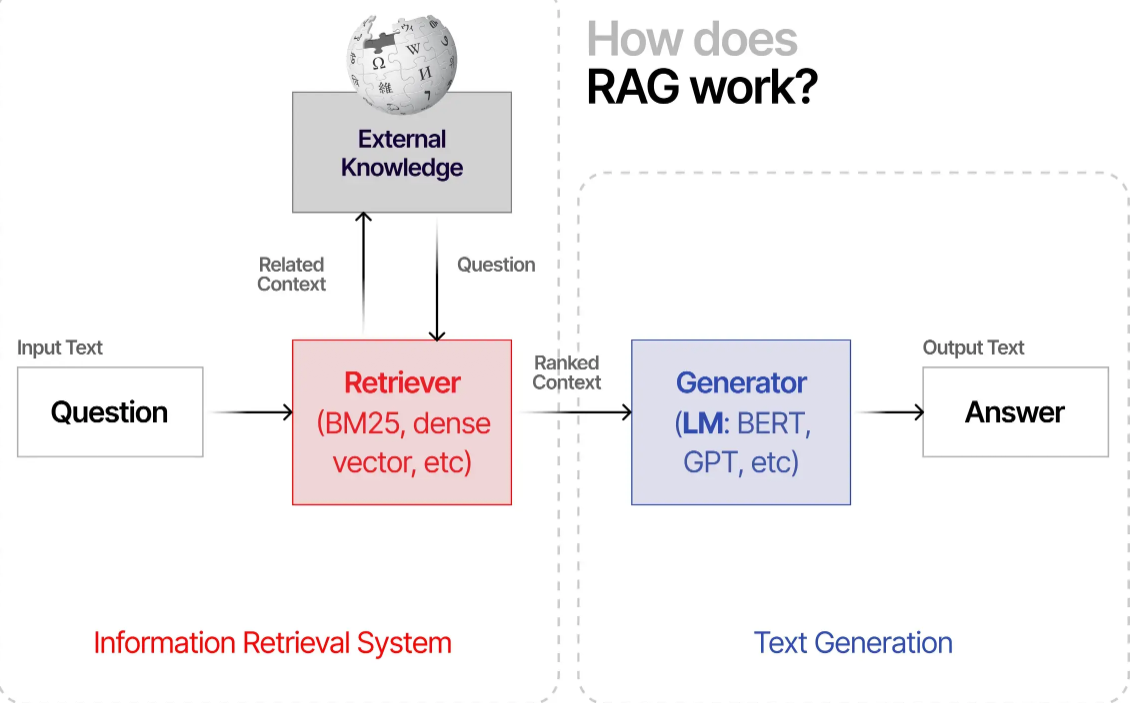
\includegraphics[width=0.9\textwidth]{rag.JPG}
		\caption{RAG system component\cite{gupta20241}. }\label{rag.PNG}
	\end{figure}
	As illustrated in figure \ref{rag.PNG}, the RAG system is built around two main components: the retriever and the generator. The retriever's role is to find relevant information from a pre-built data store, while the generator utilizes this retrieved data to produce coherent and contextually appropriate content. The overall RAG process operates as follows :
	\subsection{Retrieval in RAG Systems}\label{subsec2}
	
	Retrieval is the process of identifying and gathering information system resources that match a specific information need. To break it down, imagine these resources as a key-value store, represented as pairs:
	
	\begin{equation}
	\{(k_i, v_i)\}_{i=1}^{N}
	\end{equation}
	
	where each key \( k_i \) is linked to a corresponding value \( v_i \) (often, the key and value are the same). When a query \( q \) is provided, the goal is to find the top-\( k \) keys that are most similar to the query using a similarity function \( s \), and then retrieve their associated values\cite{gupta20241}.
	
	Depending on the similarity function used, retrieval methods can be grouped into categories such as sparse retrieval\cite{bai2020spartermlearningtermbasedsparse}which relies on exact term matching techniques like BM25 and TF-IDF, dense retrieval\cite{karpukhin2020dpr}which Uses deep learning models to encode queries and documents into dense vector embeddings, retrieving relevant documents based on semantic similarity rather than exact word matching, and others. For the widely used sparse and dense retrieval approaches, the process typically involves two main steps:  \\
	1. Encoding each object into a specific representation (e.g., term-based for sparse retrieval, vector embeddings for dense retrieval).\\
	2. Building an index to organize and efficiently retrieve relevant data during search .
	
	This structured approach ensures that the most relevant information is retrieved quickly and accurately\cite{zhao2024retrievalaugmentedgenerationaigeneratedcontent}.
	
	\subsection{Generator  in RAG Systems}\label{subsec2}
	In Retrieval-Augmented Generation (RAG) systems, the generator\cite{huang2024surveyretrievalaugmentedtextgeneration} is a key component responsible for crafting the final output. It works by combining the retrieved information with the users input query to produce a well-structured and contextually relevant response.
	
	Once the retriever fetches relevant data from external sources,the generator processes and integrates this information into a well-structured and meaningful  response. At the core of this process is a Large Language Model (LLM), which ensures that the generated text is not only fluent and accurate but also remains relevant to the original query.
	
	In various generative tasks, different models are selected based on the specific requirements: Models like BART\cite{lewis2019bart}, GPT\cite{brown2020language}and and T5 \cite{raffel2020exploring} are commonly used for tasks such as text summarization and translation, Vision-Language Models (VLMs) \cite{radford2021learningtransferablevisualmodels} are employed to generate textual descriptions from images, for text-to-Code Generation: Models like OpenAIs Codex \cite{chen2021evaluatinglargelanguagemodels} are designed to translate natural language prompts into executable code.
	
	
	\section{dyRAG: The proposed Solution}\label{sec3}
	In traditional candidate selection systems, the reliance on static or fixed top-K retrieval lead to suboptimal retrieval performance, especially in scenarios where the relevance distribution of candidates is highly variable. In this section, we introduce the Mixture of Logits (MoL) and describe its role in representing a learned similarity function. Table \ref{tab:Notations_table} summarizes the notations used in this paper and we propose Dynamic Candidate Selection, a novel algorithm that adaptively refines the candidate selection process by leveraging component-level embeddings and a Mixture of Logits (MoL) scoring mechanism.
	
	\begin{table}[h]
		\centering
		\large  % Increase overall font size
		\begin{tabular}{|c|p{10cm}|}  % Use p{width} for text wrapping
			\hline
			\textbf{Notation} & \textbf{Description} \\ \hline
			\( q \) (\( Q \), \( |Q| \)) & A single query (set of all queries, total number of queries). \\ \hline
			\( x \) (\( X \), \( |X| \)) & A single item (set of all items, total number of items). \\ \hline
			\( \phi(q, x) \) & The learned similarity function, Mixture-of-Logits (MoL), which computes the similarity between \( q \) and \( x \). \\ \hline
			\( P \) (\( P_q \), \( P_x \)) & Total number of low-rank embeddings (\( P = P_q \times P_x \)), where \( P_q \) and \( P_x \) are the number of embeddings for \( q \) and \( x \), respectively. \\ \hline
			\( \pi_p(q, x) \)  & Weight for the \( p \)-th (or \( p_q \)-th and \( p_x \)-th) embedding set for \( (q, x) \). \\ \hline
			\( f(q) \) (\( f_p(q) \)) & Learned embedding for the query (\( p \)-th component-level embedding for \( q \)). \\ \hline
			\( g(x) \) (\( g_p(x) \)) & Learned embedding for the item (\( p \)-th component-level embedding for \( x \)). \\ \hline
			\( \langle f(q), g(x) \rangle \) & Dot product similarity function: \( \langle f(q), g(x) \rangle = g(x)^T f(q) \). \\ \hline
		\end{tabular}
		\caption{Notation Table }
		\label{tab:Notations_table}
	\end{table}
	
	
	\subsection{Mixture of Logits} 
	
	The Mixture of Logits (MoL)\cite{zhai2023revisiting,ding2024efficient} methode provides a flexible and adaptive mechanism for computing similarity scores between queries and items. Given a query \( q \) and an item \( x \), MoL assumes that both are mapped to \( P \) groups of low-rank embeddings, denoted as \( f_p(q) \) and \( g_p(x) \), respectively. These embeddings are parameterized by neural networks that extract features from the query and item. The similarity between \( q \) and \( x \) is computed as a weighted sum of the inner products of these embeddings, where the weights \( \pi_p(q, x) \)\cite{zhai2023revisiting,ding2024efficient} are adaptive gating parameters constrained to sum to 1:
	
	\begin{equation}
	\text{Similarity}(q, x) = \sum_{p=1}^P \pi_p(q, x) \cdot \langle f_p(q), g_p(x) \rangle.
	\end{equation}
	
	This formulation allows MoL to capture complex relationships between queries and items, making it particularly suitable for dynamic candidate selection tasks.
	
	To efficiently scale MoL for large datasets and hardware-optimized implementations, the formulation is extended by decomposing the dot products into batched outer products of query-side and document-side embeddings. This decomposition improves computational efficiency, particularly on accelerators like GPUs, by normalizing the embeddings using the \( l_2 \)-norm:\cite{zhai2023revisiting}
	
	\begin{equation}
	\phi(q,x) = \sum_{pq=1}^{P_q} \sum_{px=1}^{P_x} \pi_{pq,px}(q,x) \frac{\langle f_{pq}(q), g_{px}(x) \rangle}{|| f_{pq}(q) ||_2 || g_{px}(x) ||_2}
	\end{equation}
	
	
	Since embedding normalization can be precomputed, both formulations remain interchangeable in practical applications. Furthermore, it is possible to decompose any high-rank matrix into a mixture of logits based on low-rank matrices, demonstrating the flexibility and scalability of this approach in large-scale information retrieval tasks. 
	
	\subsection{Retrieval Algorithm}
	We propose an \textbf{adaptive threshold mechanism} (referred to as (Dynamic Candidate Selection) that leverages the Mixture of Logits (MoL) framework to enhance the candidate retrieval process. The mechanism operates as follows:
	
	\noindent
	1. \textbf{Component-Level Embeddings}:  
	Component-level embeddings are generated for all items in the dataset \(X\). These embeddings facilitate efficient similarity computations during retrieval. Formally,
	\begin{equation}
	X_p \leftarrow \{g_p(x) \mid x \in X\}.
	\end{equation}
	
	\noindent
	2.\textbf{ Initial Candidate Retrieval:} This step involves computing similarity scores between a query representation and item representations for each feature component $p \in P$.  
	
	\begin{equation}
	S_p \gets  \{ \langle f_p(q), g_p(x) \rangle : x \in X_p \}
	\label{eq:initial_retrieval}
	\end{equation}
	Here, $f_p(q)$ and $g_p(x)$ represent the feature embeddings of the query $q$ and item $x$ for the $p$-th component, respectively. The dot product $\langle f_p(q), g_p(x) \rangle$ measures the relevance of each item $x \in X_p$ with respect to $q$, producing a set of scores $S_p$ .
	
	
	\noindent
	3. \textbf{Dynamic Threshold Adjustment}:  
	To improve retrieval quality, \textbf{Mixture of Logits (MoL)} scores are computed for each candidate \(x \in G\). The adaptive gating weights \(\pi_p(q, x)\) allow the algorithm to dynamically adjust the retrieval threshold \(T_{\text{adaptive}}\) based on the MoL scores. The scoring function is defined as:
	\begin{equation}
	\phi(q, x) = \sum_{p=1}^{P} \pi_p(q, x) \cdot \langle f_p(q), g_p(x) \rangle.
	\label{similarity_function}
	\end{equation}
	The adaptive threshold \(T_{\text{adaptive}}\) is set as the minimum score among the candidates:
	\begin{equation}
	T_{\text{adaptive}} = \min\{s \mid s \in G\}.
	\end{equation}
	
	\noindent
	4. \textbf{Refinement and Top-K Selection}:  
	Using the adaptive threshold \(T_{\text{adaptive}}\), additional relevant candidates are retrieved, expanding the candidate set \(G'\). This is achieved by including candidates whose scores exceed the threshold:
	\begin{equation}
	G' \leftarrow G \cup \{x \mid s_p \geq T_{\text{adaptive}}\}.
	\end{equation}
	The algorithm then sorts \(G'\) based on MoL scores to select the most relevant top-k candidates.
	
	\noindent
	4. \textbf{Exact Top-K Selection}:  
	Finally, the candidates in \(G'\) are sorted by their MoL scores, and the exact top-k items are extracted:
	\begin{equation}
	G_{\text{final}} = \text{Top-k}(G', \phi(q, x)).
	\end{equation}
	As shown in Algorithm\ref{ALgo1}, the retrieval process dynamically adjusts the threshold based on MoL scores.
	\begin{algorithm}
		\caption{Hybrid Exact Top-k with Threshold-Based k Selection}
		\label{ALgo1}
		\textbf{Input:} Query $q$, Set of items $X$, Component-level embeddings: $f_p(q)$, $g_p(x)$ for $p \in P$, $x \in X$, Initial threshold $T_{\text{init}}$ \\
		\textbf{Output:} Exact top $k$ items based on dynamic threshold   selection, $G_{\text{final}}$
		
		\begin{algorithmic}[1]
			
			
			\State Set $G \gets \emptyset$     \Comment{Initial candidate set}
			\For{each component $p \in P$}
			\State $X_p \gets \{g_p(x) \mid x \in X\}$ \Comment{Precompute embeddings}
			\EndFor
			
			\textbf{1. Initial Candidate Retrieval:}
			\For{each component $p \in P$}
			\State Compute dot product scores:  with (eq\eqref{eq:initial_retrieval})
			
			\State Retrieve items with scores $S_p \geq T_{\text{init}}$
			\State Add these items to $G$
			\EndFor
			
			\textbf{2. Adjust k Dynamically:}
			\For{each $x \in G$}
			\State Compute MoL scores $s \gets \phi(q, x)$ using : eq\eqref{similarity_function}
			\State Set $T_{\text{adaptive}} = \min \{s : s \in G\}$
			\EndFor
			
			\textbf{3. Refine Candidate Set with Adaptive k:}
			\State	$G' \gets \emptyset$
			\For{each component $p \in P$}
			\State Retrieve items from $X_p$ with scores $S_p \geq T_{\text{adaptive}}$
			\State Add these items to $G'$
			\EndFor
			
			\textbf{4. Select Exact Top-k Items:}
			\For{each component $p \in P$}
			\State Compute MoL scores for all items in $G'$
			\State Sort $G'$ by MoL scores in descending order
			\State Select the top $k$ items from $G'$ where $k$ is the number of items in $G'$ exceeding $T_{\text{adaptive}}$
			\EndFor
			\State\textbf{ Return:} $G_{\text{final}}$ \Comment{Retrieve Top $k$ items from $G'$}
		\end{algorithmic}
	\end{algorithm}
	\newpage
	\subsection{Evaluation metrics in recommendation system}
	
	The retrieval algorithm is integrated into a recommendation system, and its effectiveness is assessed using standard ranking metrics. These metrics are widely used in sequential recommendation tasks to evaluate the model's ability to rank relevant items higher in a user's preference list:
	
	\begin{itemize}
		\item \textbf {Hit Rate at \( K \)} (HR@K) evaluates the proportion of users who have at least one relevant item in their top-\( K \) recommendations. It is computed as \cite{eviden2025mrr}:
		
		\begin{equation}
		HR@k = \frac{1}{|U|} \sum_{u \in U} I(|\text{rel}(u) \cap \text{rec}_k(u)| > 0)
		\end{equation}
		
		where \( \text{rel}(u) \) denotes the relevant items for user \( u \), \( \text{rec}_k(u) \) represents the top-\( K \) recommended items, and \( I(\cdot) \) is an indicator function that returns 1 if at least one relevant item is present in the recommendations, otherwise 0.  
		
		HR@K can be evaluated at different values of \( K \) (e.g., 3, 5, 10) to assess model performance across various ranking depths.
		
		\item \textbf{Mean Reciprocal Rank (MRR)}:is a ranking quality metric that measures how quickly a system retrieves the first relevant item. It is calculated as the average of reciprocal ranks across all users or queries,MRR ranges from 0 to 1, with higher values indicating better performance \cite{eviden2025mrr}.
		\begin{equation}
		\text{MRR} = \frac{1}{|U|} \sum_{u=1}^{|U|} \frac{1}{\text{rank}_u},
		\end{equation}
		where \( \text{rank}_u \) is the position of the first relevant item for user \( u \) within the top-K results. \\ 
		U represents the total number of users (for recommendation systems) or queries (for information retrieval tasks) in the dataset.
		
		\item \textbf{Normalized Discounted Cumulative Gain (NDCG)}: Assesses the ranking quality while accounting for position importance. The NDCG@\( k \) is computed as:\cite{eviden2025mrr}
		\begin{equation}
		\text{NDCG@}k = \frac{1}{|U|} \sum_{u=1}^{|U|} \frac{\text{DCG@}k}{\text{IDCG@}k},
		\end{equation}
		where \( \text{DCG@}k \) is the Discounted Cumulative Gain at position \( k \):
		\begin{equation}
		\text{DCG@}k = \sum_{i=1}^{k} \frac{2^{\text{rel}_i} - 1}{\log_2(i + 1)},
		\end{equation}
		and \( \text{IDCG@}k \) is the Ideal DCG@\( k \), computed by sorting the items by their true relevance scores.
	\end{itemize}  
	\section{Experimental Results}\label{sec3}
	In order to measure the effectiveness of our proposed method, we perform a comprehensive evaluation of both the retrieval algorithm and the Mixture-of-Logits (MoL) approach. This assessment focuses on the next-item prediction task, a fundamental challenge in recommendation systems\cite{Zhu_2018}\cite{kang2018selfattentivesequentialrecommendation}, where the goal is to predict the most relevant item a user will interact with next based on their past interactions. 
	\subsection{Dataset description}
	We conducted experiments using two MovieLens datasets : ML-100K and ML-1M \cite{Harper2015}which are widely used benchmarks for evaluating sequential recommendation models as detailed in Table\ref{tab:movielens}.\\
	\begin{table}[h]
		\centering
		\renewcommand{\arraystretch}{1.2}
		\begin{tabular}{|l|p{10cm}|}
			\hline
			\textbf{Dataset} & \textbf{Description} \\
			\hline
			\textbf{MovieLens-100K} & 100,000 ratings (1-5 scale) from 943 users on 1,682 movies. \\
			& Each user has rated at least 20 movies. \\
			& Includes user demographic information (age, gender, occupation, zip code). \\
			\hline
			\textbf{MovieLens-1M} & 1,000,209 ratings from 6,040 users on approximately 3,900 movies. \\
			& Data collected from users who joined MovieLens in 2000. \\
			& Represents a larger-scale recommendation scenario. \\
			\hline
		\end{tabular}
		\caption{Summary of MovieLens datasets}
		\label{tab:movielens}
	\end{table}
	\subsection{ Experiments Setup }
	For both datasets, We utilize the SASRec architecture as our sequential user encoder, a model renowned for achieving state-of-the-art performance in next-item prediction tasks. This architecture processes the user's historical interaction sequence, generating embeddings that encapsulate the user's preferences at each time step. These embeddings serve as the foundation for predicting the next item in the sequence.
	
	The query \( q \) represents the user's state at a specific time step, derived from their interaction history. In the MoL (Mixture of Logits) framework,\( q \)is transformed into \( Pq \)
	embeddings through a multi-layer perceptron (MLP).
	\subsection{Impact of Hyperparameters}
	For fair comparison, we maintained consistent architectural choices and training conditions across all experiments, We conducted an extensive hyperparameter analysis comparing both approaches (Hybrid+SAS and MoL+SAS) across different architectural configurations. All experiments were Implemented in TensorFlow and trained on a Google Colab environment with a T4 GPU. We use the Adam optimizer with a learning rate of 0.001. For the hybrid algorithm, we initialize the threshold (Tinit) to 0.3 and adaptively adjust it during training. We discuss detailed hyperparameter settings in table \ref{tab:100k_movies}, table \ref{tab:1m_movies}
	
	
	\setlength{\tabcolsep}{1pt} % Increase column padding
	
	\begin{table}[ht]
		\centering
		\large
		\renewcommand{\arraystretch}{1.7} % Increase row spacing
		\resizebox{\textwidth}{!}{  % Scale table to fit width
			\begin{tabular}{|l|c|c|c|c|c|c|c|c|}
				\hline
				\textbf{Model} & \textbf{\shortstack{Max \\ Sequence Length}} & 
				\textbf{\shortstack{Embedding \\ Dimension}} & 
				\textbf{\shortstack{Number \\ of Heads}} & 
				\textbf{\shortstack{Feedforward \\ Dimension}} & 
				\textbf{\shortstack{Batch \\ Size}} & 
				\textbf{Epochs} & 
				\textbf{\shortstack{Val \\ Loss}} & 
				\textbf{\shortstack{Val \\ Accuracy}} \\
				\hline
				Hybrid+SAS & 50  & 128  & 2 & 128  & 128 & 12 & 5.3036 & 0.1584  \\ \hline
				MoL+SAS    & 50  & 128  & 2 & 128  & 128 & 12 & 5.3152 & 0.1582  \\ \hline
				Hybrid+SAS & 128 & 256  & 4 & 256  & 128 & 10 & 3.6364 & 0.4301  \\ \hline
				MoL+SAS    & 128 & 256  & 4 & 256  & 128 & 10 & 3.6374 & 0.4299 \\\hline
				Hybrid+SAS & 512 & 512  & 4 & 512  & 128 & 10 & 1.2808 & {\bf 0.8120} \\ \hline
				MoL+SAS    & 512 & 512  & 4 & 512  & 128 & 10 & 1.3050 & 0.8016 \\\hline
			\end{tabular}
		}
		\caption{Results on 100kMovies dataset}
		\label{tab:100k_movies}
	\end{table}
	
	
	\setlength{\tabcolsep}{1pt} % Increase column padding
	
	\begin{table}[ht]
		\centering
		\large
		\renewcommand{\arraystretch}{1.7} % Increase row spacing
		\resizebox{\textwidth}{!}{  % Scale table to fit width
			\begin{tabular}{|l|c|c|c|c|c|c|c|c|}
				\hline
				\textbf{Model} & \textbf{\shortstack{Max \\ Sequence Length}} & 
				\textbf{\shortstack{Embedding \\ Dimension}} & 
				\textbf{\shortstack{Number \\ of Heads}} & 
				\textbf{\shortstack{Feedforward \\ Dimension}} & 
				\textbf{\shortstack{Batch \\ Size}} & 
				\textbf{Epochs} & 
				\textbf{\shortstack{Val \\ Loss}} & 
				\textbf{\shortstack{Val \\ Accuracy}} \\
				\hline
				Hybrid+SAS & 50  & 128  & 2 & 128  & 128 & 10 & 4.5721 & 0.1530  \\ \hline
				MoL+SAS    & 50  & 128  & 2 & 128  & 128 & 10 & 4.5733 & 0.1526  \\ \hline
				Hybrid+SAS & 128 & 256  & 4 & 256  & 128 & 10 & 3.4152 & 0.3680  \\ \hline
				MoL+SAS    & 128 & 256  & 4 & 256  & 128 & 10 & 3.4671 & 0.3627  \\ \hline
				Hybrid+SAS & 512 & 512  & 4 & 512  & 128 & 10 & 1.0275 & {\bf 0.8350} \\ \hline
				MoL+SAS    & 512 & 512  & 4 & 512  & 128 & 10 & 1.0350 & 0.8276  \\ \hline
				
			\end{tabular}
		}
		\caption{Results on 1M Movies dataset}
		\label{tab:1m_movies}
	\end{table}
	\newpage
	Both approaches demonstrate significant performance improvements as model capacity increases, with larger configurations consistently delivering better results. For instance, when increasing the model's capacity such as expanding the (Max Sequence Length: 512, Embedding Dimension: 512, Number of Heads: 4, Feed-Forward Dimension: 512) the hybrid algorithm combined with SASRec (Hybrid+SAS) achieves notable gains, particularly in the most resource-intensive setup. On the ML-100K dataset, Hybrid+SAS reaches a score of\textbf{0.8120} compared to the baseline's \textbf{0.8016}, while on ML-1M, it achieves \textbf{0.8350} versus \textbf{0.8276} The ML-1M dataset generally benefits more from increased capacity, with the performance gap between datasets narrowing as the model scales. While smaller configurations provide a balance of efficiency and performance, the largest configuration, despite its higher computational demands, yields the best results, making it suitable for scenarios where resources are not a constraint. Both approaches show similar benefits from scaling, but Hybrid+SAS maintains a consistent edge in performance.
	
	As shown in Figures~\ref{fig:k_changes_100K} and \ref{fig:k_changes_1M}, the value of $k$ fluctuates across epochs for both MovieLens 100K and MovieLens 1M datasets. These variations indicate the adaptive nature of $k$ in response to the dataset characteristics and training progress. In the following section, we analyze how these changes influence model performance.  
	
	\begin{figure}[htbp]
		\centering
		\begin{subfigure}{0.48\textwidth}
			\centering
			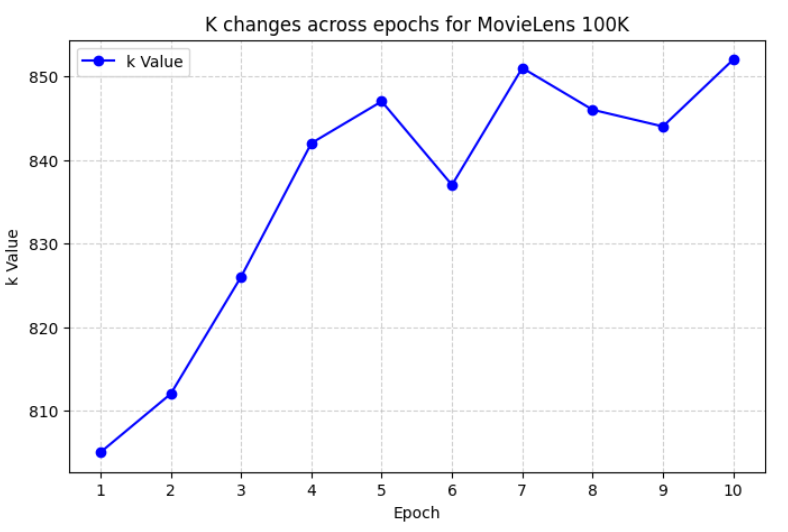
\includegraphics[width=\linewidth]{CHAGES_OF_K_FOR_100k.png}
			\caption{K changes across epochs for MovieLens 100K}
			\label{fig:k_changes_100K}
		\end{subfigure}
		\hfill
		\begin{subfigure}{0.48\textwidth}
			\centering
			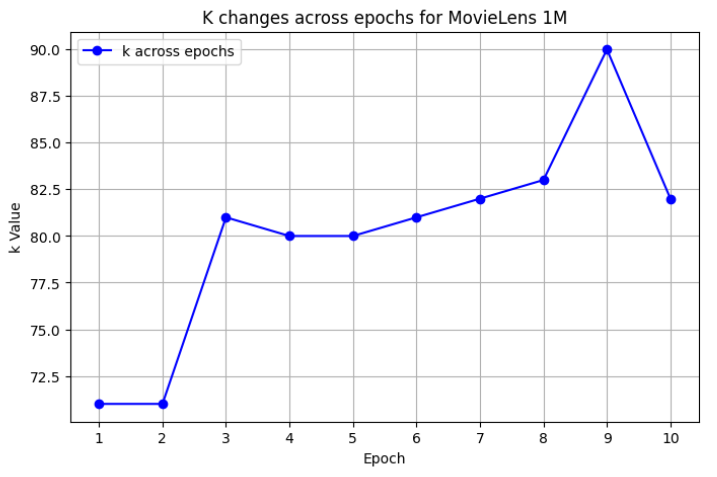
\includegraphics[width=\linewidth]{chnages_inK_for_1M.png}
			\caption{K changes across epochs for MovieLens 1M}
			\label{fig:k_changes_1M}
		\end{subfigure}
		\caption{Comparison of K changes across epochs for different datasets}
		\label{fig:k_changes}
	\end{figure}
	the value of K changed dynamically during training, with different behaviors. For the MovieLens 100K dataset, K showed a steady increase across epochs, whereas for the MovieLens 1M dataset, K began at a lower value, experienced fluctuations, peaked, and then stabilized. This indicates that the larger dataset necessitated more adaptive adjustments in retrieval compared to the smaller dataset.\\
	Figure~\ref{histo_p} summarizes the performance of our hybrid algorithm compared to the MoL-based approach on the MovieLens 100K and 1M datasets, both tested using a Max Sequence Length of 50, an Embedding Dimension of 128, 2 Attention Heads, a Feedforward Dimension of 128, a Batch Size of 128, and trained for 10 epochs . \\
	\begin{figure}[ht]
		\centering
		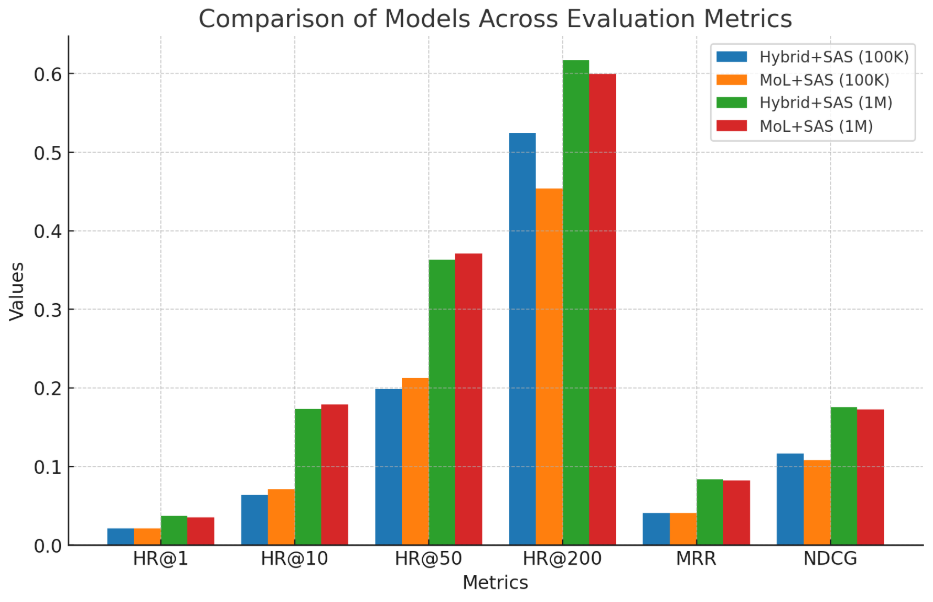
\includegraphics[width=0.7\textwidth]{HISTOGRAM.png}
		\caption{Comparison of Models Across Evaluation Metrics}\label{histo_p}
	\end{figure}
	The variations in K help explain the performance differences seen in the fig \ref{histo_p}. The Hybrid+SAS model applied to the MovieLens 1M dataset, which exhibited more dynamic changes in K achieved higher HR@50(0.3631) and HR@200(0.6170) scores, reflecting better long-range recommendation quality. The fluctuations in K in the 1M dataset likely allowed the model to balance exploration and precision, improving its overall ranking performance.
	
	On the other hand, the more gradual K increase in the 100K dataset resulted in relatively lower scores, suggesting that a static or overly conservative 
	K selection might limit retrieval effectiveness.
	
	Additionally, the MoL+SAS model achieved better performance than Hybrid+SAS in HR@10 for both datasets. This aligns with the observation that MoL+SAS tended to retrieve fewer but more relevant items at shorter ranking positions. This behavior can be attributed to how K evolved during training?smaller K values in earlier epochs likely enabled MoL+SAS to maintain higher precision at shorter ranks.
	These findings highlight the importance of dynamically tuning K based on dataset characteristics to optimize recommendation effectiveness.
	
	
	The results demonstrate that the Hybrid Exact Top-k algorithm effectively leverages both sequential user behavior and item metadata to improve recommendation quality. The adaptive MoL threshold allows the model to dynamically refine candidate items during training, leading to better performance. The improvements are consistent across both datasets, highlighting the robustness of our approach.\\
	%%=============================================%%
	%% For presentation purpose, we have included  %%
	%% \bigskip command. Please ignore this.       %%
	%%=============================================%%
	\bigskip
	\begin{minipage}{\hsize}%
		\lstset{frame=single,framexleftmargin=-1pt,framexrightmargin=-17pt,framesep=12pt,linewidth=0.98\textwidth,language=pascal}% Set your language (you can change the language for each code-block optionally)
		%%% Start your code-block
		
	\end{minipage}
	
	%Here is an example for \verb+\cite{...}+: \cite{bib1}. Another example for %\verb+\citep{...}+: \citep{bib2}. For author-year citation mode, \verb+\cite{...}+ %prints Jones et al. (1990) and \verb+\citep{...}+ prints (Jones et al., 1990).
	
	%All cited bib entries are printed at the end of this article: \cite{bib3}, %\cite{bib4}, \cite{bib5}, \cite{bib6}, \cite{bib7}, \cite{bib8}, \cite{bib9}, %\cite{bib10}, \cite{bib11}, \cite{bib12} and \cite{bib13}.
	%%=============================================%%
	%% For presentation purpose, we have included  %%
	%% \bigskip command. Please ignore this.       %%
	%%=============================================%%
	
	\section{Conclusion}\label{sec13}
	
	Choosing the right value for K in retrieval-based systems is a significant challenge, as it directly impacts both the efficiency and accuracy of information retrieval. While using a fixed K is straightforward, it often fails to adapt to the varying complexities of different queries. This can result in either missing important information or retrieving irrelevant data, which adds noise to the results. On the other hand, dynamically adjusting K offers greater flexibility but comes with its own set of challenges, such as increased computational costs and inconsistencies in determining the optimal retrieval size.
	
	To address these limitations, we introduced a hybrid dynamic K selection strategy that strikes a balance between adaptability and efficiency. Our approach adjusts K based on the unique characteristics of each query while keeping computational demands manageable. This method has shown promising results, improving retrieval performance by minimizing unnecessary noise and ensuring that critical information is consistently captured.
	
	Future work can explore enhancing our model with learning-based retrieval strategies such as reinforcement learning or attention mechanisms could refine the dynamic selection of K Additionally, testing our approach in real-world scenarios and conducting large-scale evaluations across diverse domains will help validate its robustness and adaptability in various knowledge bases and retrieval settings.
	
	
	
	
	\newpage
	
	%%===================================================%%
	%% For presentation purpose, we have included        %%
	%% \bigskip command. Please ignore this.             %%
	%%===================================================%%
	
	
	%%===========================================================================================%%
	%% If you are submitting to one of the Nature Portfolio journals, using the eJP submission   %%
	%% system, please include the references within the manuscript file itself. You may do this  %%
	%% by copying the reference list from your .bbl file, paste it into the main manuscript .tex %%
	%% file, and delete the associated \verb+\bibliography+ commands.                            %%
	%%===========================================================================================%%
	
	\bibliography{sn-bibliography}% common bib file
	%% if required, the content of .bbl file can be included here once bbl is generated
	%%\input sn-article.bbl
	
	
\end{document}
